\documentclass[aspectratio=169]{beamer}
\usepackage[portuges]{babel}
\usepackage[utf8]{inputenc}
\usepackage[alf]{abntex2cite}	
\usepackage[portuguese, linesnumbered, vlined, titlenumbered, ruled]{algorithm2e}
\usepackage{beamerthemesplit}
\usepackage{multirow}
\usepackage{scalefnt}
\SetKwRepeat{Registro}{registro \{}{\}}%
\newcommand{\Int}{\KwSty{int}}

\usepackage{tikz}
\usetikzlibrary{matrix,backgrounds,matrix,positioning,arrows}
\usetikzlibrary{patterns,arrows,decorations.pathreplacing}
% The Beamer class comes with a number of default slide themes
% which change the colors and layouts of slides. Below this is a list
% of all the themes, uncomment each in turn to see what they look like.

%\usetheme{default}
%\usetheme{AnnArbor}
%\usetheme{Antibes}
%\usetheme{Bergen}
%\usetheme{Berkeley}
%\usetheme{Berlin}
%\usetheme{Boadilla}
%\usetheme{CambridgeUS}
%\usetheme{Copenhagen}
%\usetheme{Darmstadt}
%\usetheme{Dresden}
%\usetheme{Frankfurt}
%\usetheme{Goettingen}
%\usetheme{Hannover}
%\usetheme{Ilmenau}
%\usetheme{JuanLesPins}
%\usetheme{Luebeck}
\usetheme{Madrid}
%\usetheme{Malmoe}
%\usetheme{Marburg}
%\usetheme{Montpellier}
%\usetheme{PaloAlto}
%\usetheme{Pittsburgh}
%\usetheme{Rochester}
%\usetheme{Singapore}
%\usetheme{Szeged}
%\usetheme{Warsaw}

% As well as themes, the Beamer class has a number of color themes
% for any slide theme. Uncomment each of these in turn to see how it
% changes the colors of your current slide theme.

%\usecolortheme{albatross}
%\usecolortheme{beaver}
%\usecolortheme{beetle}
%\usecolortheme{crane}
\usecolortheme{dolphin}
%\usecolortheme{dove}
%\usecolortheme{fly}
%\usecolortheme{lily}
%\usecolortheme{orchid}
%\usecolortheme{rose}
%\usecolortheme{seagull}
%\usecolortheme{seahorse}
%\usecolortheme{whale}
%\usecolortheme{wolverine}

%\setbeamertemplate{footline} % To remove the footer line in all slides uncomment this line
%\setbeamertemplate{footline}[page number] % To replace the footer line in all slides with a simple slide count uncomment this line

%\setbeamertemplate{navigation symbols}{} % To remove the navigation symbols from the bottom of all slides uncomment this line


\usepackage{graphicx} % Allows including images
\usepackage{booktabs} % Allows the use of \toprule, \midrule and \bottomrule in tables

%%%%%%%%%%%%%%%%%%%%%%%%%%%%%%%%%%%%%%%%%%%%%%%%%%%%%%%%%%%%%%%%%%%%%%%%%%%%%%%%%%%%%%%%%
%	TITLE PAGE
%%%%%%%%%%%%%%%%%%%%%%%%%%%%%%%%%%%%%%%%%%%%%%%%%%%%%%%%%%%%%%%%%%%%%%%%%%%%%%%%%%%%%%%%%

\title[Algoritmos de Ordenação]{Algoritmos e Estrutura de Dados II}
\subtitle{Algoritmos de Ordenação}
\author[Frederico Santos de Oliveira]{prof. Frederico Santos de Oliveira}
\institute[UFMT]{Universidade Federal de Mato Grosso\\ Instituto de Engenharia}
\date{}
\begin{document}

%%%%%%%%%%%%%%%%%%%%%%%%%%%%%%%%%%%%%%%%%%%%%%%%%%%%%%%%%%%%%%%%%%%%%%%%%%%%%%%%%%%%%%%%%

\begin{frame}
\titlepage % Print the title page as the first slide

\begin{figure}[!h]
  \centering
  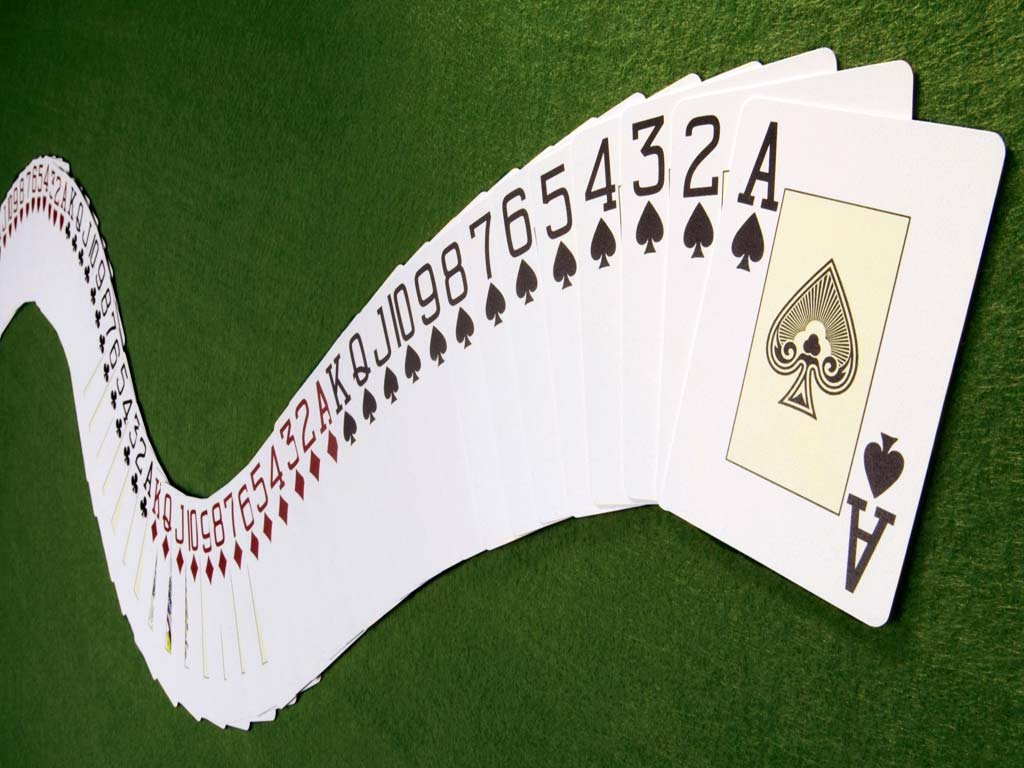
\includegraphics[width=120pt]{imgs/introducao.jpg}
  \label{fig_introducao}
\end{figure}
\end{frame}

%%%%%%%%%%%%%%%%%%%%%%%%%%%%%%%%%%%%%%%%%%%%%%%%%%%%%%%%%%%%%%%%%%%%%%%%%%%%%%%%%%%%%%%%%

\begin{frame}
\frametitle{Roteiro} % Table of contents slide, comment this block out to remove it
\tableofcontents % Throughout your presentation, if you choose to use \section{} and \subsection{} commands, these will automatically be printed on this slide as an overview of your presentation
\end{frame}

%%%%%%%%%%%%%%%%%%%%%%%%%%%%%%%%%%%%%%%%%%%%%%%%%%%%%%%%%%%%%%%%%%%%%%%%%%%%%%%%%%%%%%%%%
%	PRESENTATION SLIDES
%%%%%%%%%%%%%%%%%%%%%%%%%%%%%%%%%%%%%%%%%%%%%%%%%%%%%%%%%%%%%%%%%%%%%%%%%%%%%%%%%%%%%%%%%

%%%%%%%%%%%%%%%%%%%%%%%%%%%%%%%%%%%%%%%%%%%%%%%%%%%%%%%%%%%%%%%%%%%%%%%%%%%%%%%%%%%%%%%%%
\section{Objetivos}
%%%%%%%%%%%%%%%%%%%%%%%%%%%%%%%%%%%%%%%%%%%%%%%%%%%%%%%%%%%%%%%%%%%%%%%%%%%%%%%%%%%%%%%%%

\begin{frame}
\frametitle{Objetivos}

Esta aula tem como objetivos:

\begin{enumerate}
\item Apresentar os conceitos básicos sobre ordenação;
\item Explicitar os métodos mais simples de ordenação por comparação;
\item Exemplificar a execução dos algoritmos.
\end{enumerate}
\end{frame}

%%%%%%%%%%%%%%%%%%%%%%%%%%%%%%%%%%%%%%%%%%%%%%%%%%%%%%%%%%%%%%%%%%%%%%%%%%%%%%%%%%%%%%%%%
\section{Referências bibliográficas}
%%%%%%%%%%%%%%%%%%%%%%%%%%%%%%%%%%%%%%%%%%%%%%%%%%%%%%%%%%%%%%%%%%%%%%%%%%%%%%%%%%%%%%%%%

\frame{\frametitle{Referências bibliográficas}
  \bibliographystyle{abntex2-alf}
  \bibliography{referencias}
}

%%%%%%%%%%%%%%%%%%%%%%%%%%%%%%%%%%%%%%%%%%%%%%%%%%%%%%%%%%%%%%%%%%%%%%%%%%%%%%%%%%%%%%%%%
\section{Introdução} % Sections can be created in order to organize your presentation into discrete blocks, all sections and subsections are automatically printed in the table of contents as an overview of the talk
%%%%%%%%%%%%%%%%%%%%%%%%%%%%%%%%%%%%%%%%%%%%%%%%%%%%%%%%%%%%%%%%%%%%%%%%%%%%%%%%%%%%%%%%%

\begin{frame}
\frametitle{Introdução}
\begin{block}{Ordenar}
 Segundo \citeonline{Ziviani2011}, ordenar é o processo de rearranjar um conjunto de objetos em uma ordem ascendente ou descendente.
\end{block}
\begin{itemize}
\item A ordenação visa facilitar a recuperação posterior de itens do conjunto ordenado;
\item As técnicas de ordenação permitem apresentar um amplo de algoritmos distintos para resolver uma mesma tarefa.
\end{itemize}
\end{frame}

%%%%%%%%%%%%%%%%%%%%%%%%%%%%%%%%%%%%%%%%%%%%%%%%%%%%%%%%%%%%%%%%%%%%%%%%%%%%%%%%%%%%%%%%%

\begin{frame}
\frametitle{Introdução}
 Segundo \citeonline{Sedgewick2011}, existem três razões práticas para estudar os algoritmos de ordenação:
\begin{itemize}
\item Analisar os algoritmos de ordenação é uma introdução completa as técnicas de comparação de desempenho de algoritmos;
\item Técnicas semelhantes são eficazes no tratamento de outros problemas;
\item Muitas vezes usamos algoritmos de ordenação como ponto de partida para resolver outros problemas.
\end{itemize}
\pause
Mais importante do que esses motivos práticos é que os algoritmos são elegantes, clássicos, e eficazes.
\end{frame}

%%%%%%%%%%%%%%%%%%%%%%%%%%%%%%%%%%%%%%%%%%%%%%%%%%%%%%%%%%%%%%%%%%%%%%%%%%%%%%%%%%%%%%%%%

\begin{frame}
\frametitle{Notação}
\begin{itemize}
\item Os métodos trabalham sobre os registros de um arquivo;
\item Cada registro possui uma chave para controlar a ordenação;
\item Podem existir outros componentes em um registro;
\item Exemplo de estrutura, em C:
\begin{algorithm}[H]
\caption{TAD Registro} 
\label{pseudocodigo}
\Inicio{
 \Registro{ItemVetor}{
    \Int{} chave \;
    Ponteiro dados;
  }
}
\end{algorithm}
\item A chave é usada como critério para ordenação.
\item O ponteiro dados aponta para a informação indexada pela chave. 
\end{itemize}
% \begin{figure}[!h]
%   \centering
%   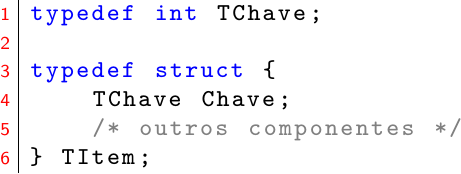
\includegraphics[width=150pt]{imgs/exemplo_registro.png}
%   \label{fig_exemplo_registro}
% \end{figure}
\end{frame}

%%%%%%%%%%%%%%%%%%%%%%%%%%%%%%%%%%%%%%%%%%%%%%%%%%%%%%%%%%%%%%%%%%%%%%%%%%%%%%%%%%%%%%%%%

\begin{frame}
\frametitle{Características}
\begin{itemize}
 \item Qualquer tipo de chave, sobre o qual exista uma regra de ordenação bem definida, pode ser utilizada;
    \begin{itemize}
     \item As ordens mais usadas são a numérica e a lexicográfica.
    \end{itemize}

 \item Um método de ordenação é \underline{estável} se a ordem relativa dos itens com chaves iguais não se altera durante a ordenação.
  \begin{itemize}
   \item Alguns dos métodos mais eficientes não são estáveis;
   \item A estabilidade pode ser forçada quando o método é não-estável.
  \end{itemize}
\end{itemize}
\end{frame}


%%%%%%%%%%%%%%%%%%%%%%%%%%%%%%%%%%%%%%%%%%%%%%%%%%%%%%%%%%%%%%%%%%%%%%%%%%%%%%%%%%%%%%%%%

\begin{frame}
\frametitle{Características}
Os métodos de ordenação podem ser classificados como:
  \begin{itemize}
   \item {\bf Ordenação interna}: o arquivo a ser ordenado \underline{cabe} todo na memória principal;
   \begin{itemize}   
      \item Qualquer registro pode ser imediatamente acessado.
   \end{itemize}
  \end{itemize}
  \begin{itemize}
    \item {\bf Ordenação externa}: o arquivo a ser ordenado \underline{não cabe} todo na memória principal;
    \begin{itemize}
      \item Registros são acessados sequencialmente ou em blocos.
    \end{itemize}
  \end{itemize}
\end{frame}

%%%%%%%%%%%%%%%%%%%%%%%%%%%%%%%%%%%%%%%%%%%%%%%%%%%%%%%%%%%%%%%%%%%%%%%%%%%%%%%%%%%%%%%%%

\begin{frame}
\frametitle{Características}
  \begin{itemize}
   \item A maioria dos métodos de ordenação é baseada em \underline{comparações} de chaves;
   \item Existem métodos que utilizam o princípio da \underline{distribuição};
   \item Exemplo: ordenar um baralho com 52 cartas, pelo valor e pelo naipe seguindo as seguintes instruções:
   \begin{itemize}
    \item Separe as cartas em 13 montes (valores das cartas);
    \item Colete os montes na ordem desejada;
    \item Distribua cada monte em 4 montes (naipes das cartas);
    \item Colete os montes na ordem desejada.
   \end{itemize}
  \item Qual é o custo desse algoritmo?
  \end{itemize}
\end{frame}

%%%%%%%%%%%%%%%%%%%%%%%%%%%%%%%%%%%%%%%%%%%%%%%%%%%%%%%%%%%%%%%%%%%%%%%%%%%%%%%%%%%%%%%%%

\begin{frame}
\frametitle{Critérios de análise}
  \begin{itemize}
   \item Dado que $n$ é a quantidade de registros em um arquivo, as medidas de complexidade relevantes são:
    \begin{itemize}
      \item número de comparações $C(n)$ entre chaves;
      \item número de movimentações $M(n)$ de registros dos arquivo.
    \end{itemize}
    \item O uso da memória é um requisito primordial na ordenação interna:
    \begin{itemize}
      \item os métodos de ordenação {\it in situ} são os preferidos;
      \item também existem aqueles que utilizam listas encadeadas;
      \item e os métodos que fazem cópias dos itens a serem ordenados.
    \end{itemize}
  \end{itemize}    
\end{frame}

%%%%%%%%%%%%%%%%%%%%%%%%%%%%%%%%%%%%%%%%%%%%%%%%%%%%%%%%%%%%%%%%%%%%%%%%%%%%%%%%%%%%%%%%%

\begin{frame}
\frametitle{Ordenação interna por comparação}
\begin{block}{Métodos simples:}
    \begin{itemize}
      \item adequados para pequenos arquivos;
      \item requerem $O(n^2)$ comparações;
      \item produzem programas pequenos.
    \end{itemize}   
\end{block}
\begin{block}{Métodos eficientes:}
   \begin{itemize}
    \item adequados para arquivos maiores;
    \item requerem $O(n \log  n  )$ comparações;
    \item usam menos comparações;
    \item as comparações são mais complexas nos detalhes.
   \end{itemize} 
\end{block}
\end{frame}

%%%%%%%%%%%%%%%%%%%%%%%%%%%%%%%%%%%%%%%%%%%%%%%%%%%%%%%%%%%%%%%%%%%%%%%%%%%%%%%%%%%%%%%%%

\begin{frame}
\frametitle{O que estudaremos?}
\begin{block}{Na disciplina:}
Estudaremos os algoritmos de {\bf ordenação interna} que utilizam o príncipio de {\bf comparação} e {\bf por contagem}.
\end{block}
\begin{block}{Nesta aula:}
   \begin{itemize}
	\item Bubblesort
	\item Selectionsort 
	\item Insertionsort
   \end{itemize} 
\end{block}
\end{frame}

%%%%%%%%%%%%%%%%%%%%%%%%%%%%%%%%%%%%%%%%%%%%%%%%%%%%%%%%%%%%%%%%%%%%%%%%%%%%%%%%%%%%%%%%%

\begin{frame}
\frametitle{O melhor algoritmo}
  \begin{block}{Atenção}
   \begin{itemize}
    \item Não existe um método de ordenação considerado superior a todos os outros.
    \item É necessário analisar o problema e, com base nas características dos dados, decidir qual método melhor se aplica à ele.
   \end{itemize}
  \end{block}
\end{frame}

%%%%%%%%%%%%%%%%%%%%%%%%%%%%%%%%%%%%%%%%%%%%%%%%%%%%%%%%%%%%%%%%%%%%%%%%%%%%%%%%%%%%%%%%%
\section{Bubblesort}
%%%%%%%%%%%%%%%%%%%%%%%%%%%%%%%%%%%%%%%%%%%%%%%%%%%%%%%%%%%%%%%%%%%%%%%%%%%%%%%%%%%%%%%%%

\begin{frame}
\Huge{\centerline{Bubblesort}}
\end{frame}

\begin{frame}
\frametitle{Bubblesort}
\begin{itemize}
\item Os elementos vão {\bf ``borbulhando''} a cada iteração do método até a posição correta para ordenação da lista;
\item Como os elementos são trocados (borbulhados) frequentemente, há um alto custo com troca de elementos.
\end{itemize}
\end{frame}

%%%%%%%%%%%%%%%%%%%%%%%%%%%%%%%%%%%%%%%%%%%%%%%%%%%%%%%%%%%%%%%%%%%%%%%%%%%%%%%%%%%%%%%%%

% \begin{frame}
% \frametitle{Pseudo-código Bubblesort}
% \begin{algorithm}[H]
% \caption{Bubblesort} 
% \label{Bubblesort}
% \Entrada{Vetor $V[0..n-1]$, tamanho $n$}
% \Saida{Vetor $V$ ordenado}
% \Inicio{
%   \Para {($i \leftarrow 1 \textrm{ até } n - 1$)} {
%     \Para {($j \leftarrow n - 1 \textrm{ decrescendo até } i$)} {
%     \Se { ($V[j] < V[j-1]$) } {
% 	Trocar $V[j] \leftrightarrow V[j-1]$
% 	}    
%     }
%   }
% }
% \end{algorithm}
% \Tiny{Adaptado de \citeonline[p. 29]{Cormen2012}.}
% \end{frame}
% 


%%%%%%%%%%%%%%%%%%%%%%%%%%%%%%%%%%%%%%%%%%%%%%%%%%%%%%%%%%%%%%%%%%%%%%%%%%%%%%%%%%%%%%%%%

\begin{frame}{Exemplo}
\begin{figure}[!h]
  \centering
  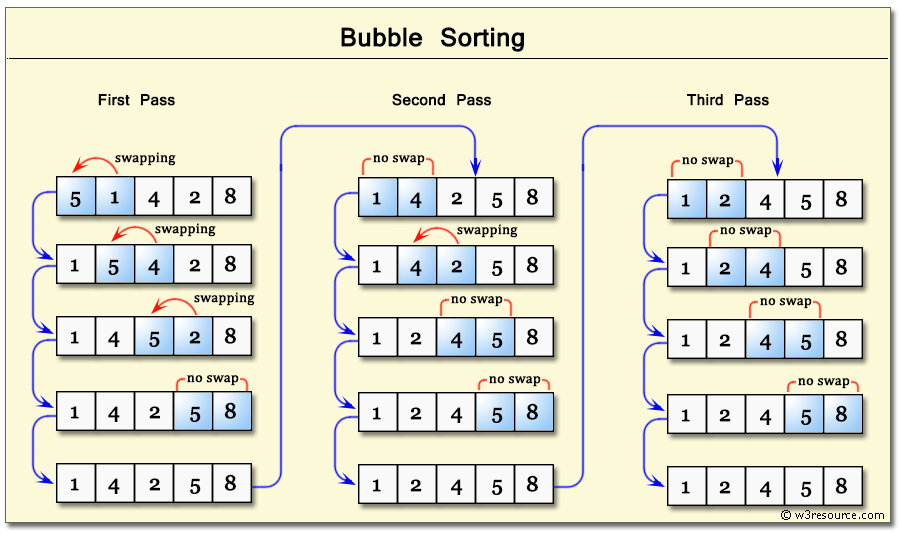
\includegraphics[width=300pt]{imgs/bubble-short.png}
  \label{fig_bubble-short}
\end{figure}
\end{frame}

%%%%%%%%%%%%%%%%%%%%%%%%%%%%%%%%%%%%%%%%%%%%%%%%%%%%%%%%%%%%%%%%%%%%%%%%%%%%%%%%%%%%%%%%%

\begin{frame}
\frametitle{Pseudo-código Bubblesort}
\begin{algorithm}[H]
\caption{Bubblesort} 
\label{Bubblesort}
\Entrada{Vetor $V[0..n-1]$, tamanho $n$}
\Saida{Vetor $V$ ordenado}
\Inicio{
  \Para {($i \leftarrow 1 \textrm{ até } n - 1$)} {
    \Para {($j \leftarrow 0 \textrm{ até } n - i - 1$)} {
    \Se { ($V[j] > V[j+1]$) } {
	Trocar $V[j] \leftrightarrow V[j+1]$
	}    
    }
  }
}
\end{algorithm}
\end{frame}

%%%%%%%%%%%%%%%%%%%%%%%%%%%%%%%%%%%%%%%%%%%%%%%%%%%%%%%%%%%%%%%%%%%%%%%%%%%%%%%%%%%%%%%%%

\begin{frame}[fragile]{Análise}{Bubblesort}
\begin{columns}[T] % align columns
\begin{column}{.55\textwidth}

\scalebox{0.8}{
\begin{algorithm}[H]
\caption{Bubblesort} 
\label{Bubblesort}
\Entrada{Vetor $V[0..n-1]$, tamanho $n$}
\Saida{Vetor $V$ ordenado}
\Inicio{
  \Para {($i \leftarrow 1 \textrm{ até } n - 1$)} {
    \Para {($j \leftarrow 0 \textrm{ até } n - i - 1$)} {
    \Se { ($V[j] > V[j+1]$) } {
	Trocar $V[j] \leftrightarrow V[j+1]$
	}    
    }
  }
}
\end{algorithm}

}
\end{column}%\frac{n^2 -n}{2}
\hfill%
\begin{column}{.45\textwidth}
Nº execuções

\end{column}%
\end{columns}
\end{frame}

%%%%%%%%%%%%%%%%%%%%%%%%%%%%%%%%%%%%%%%%%%%%%%%%%%%%%%%%%%%%%%%%%%%%%%%%%%%%%%%%%%%%%%%%%

\begin{frame}[fragile]{Análise}{Bubblesort}
\begin{columns}[T] % align columns
\begin{column}{.55\textwidth}

\scalebox{0.8}{
\begin{algorithm}[H]
\caption{Bubblesort} 
\label{Bubblesort}
\Entrada{Vetor $V[0..n-1]$, tamanho $n$}
\Saida{Vetor $V$ ordenado}
\Inicio{
  \Para {($i \leftarrow 1 \textrm{ até } n - 1$)} {
    \Para {($j \leftarrow 0 \textrm{ até } n - i - 1$)} {
    \Se { ($V[j] > V[j+1]$) } {
	Trocar $V[j] \leftrightarrow V[j+1]$
	}    
    }
  }
}
\end{algorithm}

}
\end{column}%\frac{n^2 -n}{2}
\hfill%
\begin{column}{.45\textwidth}
Nº execuções
\begin{small}
\begin{eqnarray}
L2 &=& n \nonumber \\
L3 &=& n + (n-1) + ... + 1 \nonumber \\
   &=& \frac{(1+n)(n)}{2} = \frac{n^2+n}{2} \nonumber \\
L4 &=& (n-1)+ (n-2) + ... + 0 \nonumber \\   
   &=& \frac{(0+n-1)n}{2} = \frac{n^2-n}{2} \nonumber \\
L5 &=& \frac{n^2-n}{2}  \nonumber
\end{eqnarray}
\end{small}
\end{column}%
\end{columns}
\end{frame}

%%%%%%%%%%%%%%%%%%%%%%%%%%%%%%%%%%%%%%%%%%%%%%%%%%%%%%%%%%%%%%%%%%%%%%%%%%%%%%%%%%%%%%%%%

\begin{frame}[fragile]{Análise}{Bubblesort}
\begin{table}[]
\centering
\caption{Custo Bubblesort}
\label{Custo Bubblesort}
% \scalebox{0.6}{
\begin{tabular}{c|ccc}
Linha  &  Melhor  &  Pior  &  Médio  \\
\hline
2       & n  & n  &  n \\
3       & $\frac{n^2 + n}{2}$ & $\frac{n^2 + n}{2}$ & $\frac{n^2 + n}{2}$ \\
4       &$\frac{n^2 - n}{2}$ & $\frac{n^2 - n}{2}$ & $\frac{n^2 - n}{2}$ \\
5       & 0 &$\frac{n^2 - n}{2}$& $\frac{n^2 - n}{4}$ \\ 
\end{tabular}
\end{table} 

\begin{itemize}
 \item Melhor caso: $T(n) = n + \frac{n^2+n}{2} + \frac{n^2-n}{2} + 0 = n^2 + n$

 \item Pior caso: $T(n) = n + \frac{n^2+n}{2} + 2\frac{n^2-n}{2} = \frac{3n^2}{2} + 2$
 
 \item Caso médio: $T(n) = n + \frac{n^2+n}{2} + \frac{n^2-n}{2} + \frac{n^2-n}{4} = \frac{5n^2}{4} - \frac{3n}{4}$  
\end{itemize}
\end{frame}

%%%%%%%%%%%%%%%%%%%%%%%%%%%%%%%%%%%%%%%%%%%%%%%%%%%%%%%%%%%%%%%%%%%%%%%%%%%%%%%%%%%%%%%%%

\begin{frame}[fragile]{Análise}{Bubblesort}
\begin{itemize}
 \item Número de Comparações $C(n)$ é definido pela linha 4.
 \begin{itemize}
 \item Possui custo $C(n) = \frac{n^2-n}{2}$ em qualquer situação.
 \item Portanto, o número de comparações é $C(n) = \Theta(n^2)$.
 \end{itemize}
\item Número de Movimentos $M(n)$ é definido pela linha 5.
 \begin{itemize}
 \item No melhor caso, não realiza trocas.
 \item No pior caso, realiza $\frac{n^2-n}{2}$ trocas, ou seja, é $O(n^2)$ em relação ao nº de movimentos.
 \item No caso médio, realiza $\frac{n^2-n}{4}$ trocas.
 \end{itemize} 
\end{itemize}

\end{frame}

%%%%%%%%%%%%%%%%%%%%%%%%%%%%%%%%%%%%%%%%%%%%%%%%%%%%%%%%%%%%%%%%%%%%%%%%%%%%%%%%%%%%%%%%%

\begin{frame}
\frametitle{Características}
\begin{block}{Vantagens}
  \begin{itemize}
  \item Algoritmo {\bf simples};
  \item Algoritmo {\bf estável}
  \end{itemize}
\end{block}
\begin{block}{Desvantagens}
  \begin{itemize}
  \item O fato do arquivo já estar ordenado não ajuda a reduzir o número de comparações (o custo continua quadrático), porém o número de movimentações cai para zero.
  \end{itemize} 
\end{block}
\end{frame}

%%%%%%%%%%%%%%%%%%%%%%%%%%%%%%%%%%%%%%%%%%%%%%%%%%%%%%%%%%%%%%%%%%%%%%%%%%%%%%%%%%%%%%%%%
\section{Selectionsort}
%%%%%%%%%%%%%%%%%%%%%%%%%%%%%%%%%%%%%%%%%%%%%%%%%%%%%%%%%%%%%%%%%%%%%%%%%%%%%%%%%%%%%%%%%

\begin{frame}
\Huge{\centerline{Selectionsort}}
\end{frame}

%%%%%%%%%%%%%%%%%%%%%%%%%%%%%%%%%%%%%%%%%%%%%%%%%%%%%%%%%%%%%%%%%%%%%%%%%%%%%%%%%%%%%%%%%


\begin{frame}
\frametitle{Selectionsort}
\begin{itemize}
\item A cada iteração, seleciona o menor elemento da lista e troque-o com o item na posição correta;
\item É realizada uma troca a cada iteração.
\end{itemize}
\end{frame}

%%%%%%%%%%%%%%%%%%%%%%%%%%%%%%%%%%%%%%%%%%%%%%%%%%%%%%%%%%%%%%%%%%%%%%%%%%%%%%%%%%%%%%%%%


\begin{figure}[!ht]
 \centering
  \begin{tikzpicture}
  \matrix (A)[matrix of math nodes, nodes={draw, minimum size=7mm, fill=green!30},column sep=-\pgflinewidth, column 1/.style={nodes={draw=none, fill=none, minimum size=5mm}}]
      {a) & 4 & 3 & 5 & 2 & 1 & |[fill=red!30]|0\\};     
	\draw[->] (A-1-7.north) [out=130, in=50] to (A-1-2.north);
  \begin{scope}[yshift=-1.3cm]
    \matrix(B)[matrix of math nodes, nodes={draw, minimum size=7mm, fill=green!30}, column sep=-\pgflinewidth, column 1/.style={nodes={draw=none, fill=none, minimum size=5mm}}]
	{b) & |[fill=yellow!30]|0 & 3 & 5 & 2 &  |[fill=red!30]| 1 & 4 \\};     
	\draw[->] (B-1-6.north) [out=130, in=50] to (B-1-3.north);
  \end{scope}
  \begin{scope}[yshift=-2.3cm]  
    \matrix(C)[matrix of math nodes, nodes={draw, minimum size=7mm, fill=green!30}, column sep=-\pgflinewidth, column 1/.style={nodes={draw=none, fill=none, minimum size=5mm}}]
	{c) & |[fill=yellow!30]|0 & |[fill=yellow!30]|1 & 5 & |[fill=red!30]|2 & 3 & 4\\};     
	\draw[->] (C-1-5.north) [out=130, in=50] to (C-1-4.north);
  \end{scope}
  \begin{scope}[yshift=-3.3cm]  
    \matrix(D)[matrix of math nodes, nodes={draw, minimum size=7mm, fill=green!30}, column sep=-\pgflinewidth, column 1/.style={nodes={draw=none, fill=none, minimum size=5mm}}]
	{d) & |[fill=yellow!30]|0 & |[fill=yellow!30]|1 & |[fill=yellow!30]|2 & 5 & |[fill=red!30]| 3 & 4\\};     
	\draw[->] (D-1-6.north) [out=130, in=50] to (D-1-5.north);
  \end{scope}  
  \begin{scope}[yshift=-4.25cm]  
    \matrix(E)[matrix of math nodes, nodes={draw, minimum size=7mm, fill=green!30}, column sep=-\pgflinewidth, column 1/.style={nodes={draw=none, fill=none, minimum size=5mm}}]
	{e) & |[fill=yellow!30]|0 & |[fill=yellow!30]|1 & |[fill=yellow!30]|2 & |[fill=yellow!30]|3 &  5 & |[fill=red!30]|4 \\};     
	\draw[->] (E-1-7.north) [out=130, in=50] to (E-1-6.north);
  \end{scope}    
  \begin{scope}[yshift=-5.2cm]  
    \matrix(F)[matrix of math nodes, nodes={draw, minimum size=7mm, fill=green!30}, column sep=-\pgflinewidth, column 1/.style={nodes={draw=none, fill=none, minimum size=5mm}}]
	{f) & |[fill=yellow!30]|0 & |[fill=yellow!30]|1 & |[fill=yellow!30]|2 & |[fill=yellow!30]|3 & |[fill=yellow!30]|4 & 5 \\};     
  \end{scope}        
  \end{tikzpicture}         
\label{figura_selection_sort}
\end{figure}


%%%%%%%%%%%%%%%%%%%%%%%%%%%%%%%%%%%%%%%%%%%%%%%%%%%%%%%%%%%%%%%%%%%%%%%%%%%%%%%%%%%%%%%%%


\begin{frame}
\frametitle{Pseudo-código Selectionsort}
\begin{algorithm}[H]
\caption{Selectionsort} 
\label{SelectionSort}
\Entrada{Vetor $V[0..n-1]$, tamanho $n$}
\Saida{Vetor $V$ ordenado}
\Inicio{
  \Para {$i \leftarrow 0 \textrm{ até } n-2$} {
    $min \leftarrow i$ \\
    \Para {$j \leftarrow i + 1 \textrm{ até } n-1$} {
	\Se{$V[j] < V[min]$} {
	  $min \leftarrow j$
	}
    }
    trocar $V[min] \leftrightarrow V[i]$ \\    
  }
}
\end{algorithm}
\Tiny{Adaptado de \citeonline[p. 73]{Oliveira2011}.}
\end{frame}


%%%%%%%%%%%%%%%%%%%%%%%%%%%%%%%%%%%%%%%%%%%%%%%%%%%%%%%%%%%%%%%%%%%%%%%%%%%%%%%%%%%%%%%%%

\begin{frame}[fragile]{Análise}{Selectionsort}
\begin{columns}[T] % align columns
\begin{column}{.55\textwidth}

\scalebox{0.8}{
\begin{algorithm}[H]
\caption{Selectionsort} 
\label{Selectionsort}
\Entrada{Vetor $V[0..n-1]$, tamanho $n$}
\Saida{Vetor $V$ ordenado}
\Inicio{
  \Para {$i \leftarrow 0 \textrm{ até } n-2$} {
    $min \leftarrow i$ \\
    \Para {$j \leftarrow i + 1 \textrm{ até } n-1$} {
	\Se{$V[j] < V[min]$} {
	  $min \leftarrow j$
	}
    }
    trocar $V[min] \leftrightarrow V[i]$ \\    
  }
}
\end{algorithm}

}
\end{column}%\frac{n^2 -n}{2}
\hfill%
\begin{column}{.45\textwidth}
Nº execuções



\end{column}%
\end{columns}
\end{frame}
%%%%%%%%%%%%%%%%%%%%%%%%%%%%%%%%%%%%%%%%%%%%%%%%%%%%%%%%%%%%%%%%%%%%%%%%%%%%%%%%%%%%%%%%%



\begin{frame}[fragile]{Análise}{Selectionsort}
\begin{columns}[T] % align columns
\begin{column}{.55\textwidth}

\scalebox{0.8}{
\begin{algorithm}[H]
\caption{Selectionsort} 
\label{Selectionsort}
\Entrada{Vetor $V[0..n-1]$, tamanho $n$}
\Saida{Vetor $V$ ordenado}
\Inicio{
  \Para {$i \leftarrow 0 \textrm{ até } n-2$} {
    $min \leftarrow i$ \\
    \Para {$j \leftarrow i + 1 \textrm{ até } n-1$} {
	\Se{$V[j] < V[min]$} {
	  $min \leftarrow j$
	}
    }
    trocar $V[min] \leftrightarrow V[i]$ \\    
  }
}
\end{algorithm}

}
\end{column}%\frac{n^2 -n}{2}
\hfill%
\begin{column}{.45\textwidth}
Nº execuções
\begin{small}
\begin{eqnarray}
L2 &=& n \nonumber \\
L3 &=& n - 1\nonumber \\
L4 &=& n + (n-1) + ... + 1 \nonumber \\   
   &=& \frac{(1+n)n}{2} = \frac{n^2+n}{2} \nonumber \\
L5 &=& \frac{n^2-n}{2}  \nonumber \\
L6 &=& n - 1 \nonumber
\end{eqnarray}
\end{small}
\end{column}%
\end{columns}
\end{frame}

%%%%%%%%%%%%%%%%%%%%%%%%%%%%%%%%%%%%%%%%%%%%%%%%%%%%%%%%%%%%%%%%%%%%%%%%%%%%%%%%%%%%%%%%%

\begin{frame}[fragile]{Análise}{Selectionsort}
\begin{table}[]
\centering
\caption{Custo Selectionsort}
\label{Custo Bubblesort}
% \scalebox{0.6}{
\begin{tabular}{c|ccc}
Linha  &  Melhor  &  Pior  &  Médio  \\
\hline
2       & n  & n  &  n \\
3       & n -1  & n - 1 &  n -1 \\
4       & $\frac{n^2 + n}{2}$  & $\frac{n^2 + n}{2}$  & $\frac{n^2 + n}{2}$ \\
5       & $\frac{n^2 - n}{2}$ &$\frac{n^2 - n}{2}$& $\frac{n^2 - n}{2}$ \\ 
6       & 0 &$\frac{n^2 - n}{2}$& $\frac{n^2 - n}{4}$ \\ 
7       & $n-1$ &$n-1$& $n-1$ \\ 
\end{tabular}
% }\

\begin{itemize}
 \item Melhor caso: $T(n) = n + 2(n-1) + n^2 = n^2 + 3n -2$

 \item Pior caso: $T(n) = n + 2(n-1) + \frac{n^2+n}{2} + (n^2 - n) = \frac{3n^2}{2} + \frac{5n}{2} - 2$
 
 \item Caso médio: $T(n) = n + 2(n-1) + \frac{n^2 + n}{2} + \frac{n^2 - n}{2} + \frac{n^2 - n}{4} = \frac{5n^2}{4} +\frac{11n}{4}-2$
\end{itemize}

\end{table} 
 
\end{frame}

%%%%%%%%%%%%%%%%%%%%%%%%%%%%%%%%%%%%%%%%%%%%%%%%%%%%%%%%%%%%%%%%%%%%%%%%%%%%%%%%%%%%%%%%%


\begin{frame}[fragile]{Análise}{Selectionsort}
\begin{itemize}
 \item Número de Comparações $C(n)$ é definido pela linha 5.
 \begin{itemize}
 \item Possui custo $C(n) = \frac{n^2-n}{2}$ em qualquer situação.
 \item Portanto, o número de comparações é $C(n) = \Theta(n^2)$.
 \end{itemize}
\item Número de Movimentos $M(n)$ é definido pela linha 7.
 \begin{itemize}
 \item Em qualquer situação, realiza $n-1$ trocas.
 \end{itemize} 
\end{itemize}

\end{frame}

%%%%%%%%%%%%%%%%%%%%%%%%%%%%%%%%%%%%%%%%%%%%%%%%%%%%%%%%%%%%%%%%%%%%%%%%%%%%%%%%%%%%%%%%%


\begin{frame}
\frametitle{Características}
\begin{block}{Vantagens}
  \begin{itemize}
  \item Custo linear no tamanho da entrada para o número de movimentos de registros;
  \item É o algoritmo a ser utilizado para arquivos com registros muito grandes (que possuem alto custo de movimentação);
  \item É muito interessante para arquivos pequenos.
  \end{itemize}
\end{block}
\begin{block}{Desvantagens}
  \begin{itemize}
  \item O fato do arquivo já estar ordenado não ajuda em nada, pois o custo continua quadrático;
  \item O algoritmo {\bf não é estável}.
  \end{itemize} 
\end{block}
\end{frame}

%%%%%%%%%%%%%%%%%%%%%%%%%%%%%%%%%%%%%%%%%%%%%%%%%%%%%%%%%%%%%%%%%%%%%%%%%%%%%%%%%%%%%%%%%
\section{Insertionsort}
%%%%%%%%%%%%%%%%%%%%%%%%%%%%%%%%%%%%%%%%%%%%%%%%%%%%%%%%%%%%%%%%%%%%%%%%%%%%%%%%%%%%%%%%%


\begin{frame}
\Huge{\centerline{Insertionsort}}
\end{frame}

\begin{frame}
\frametitle{Insertionsort}
\begin{itemize}
\item Algoritmo utilizado pelos jogadores de cartas:
    \begin{itemize}
      \item Inicia-se com a mão esquerda vazia e as cartas viradas com a face para baixo na mesa;
      \item Em seguida, remove-se uma carta de cada vez na mesa, inserindo-a na posição correta na mão esquerda;
      \item Para encontrar a posição correta de uma carta, compare-a sequencialmente a cada uma das cartas que já estão na mão.
      \end{itemize}      
\end{itemize}
\end{frame}

%%%%%%%%%%%%%%%%%%%%%%%%%%%%%%%%%%%%%%%%%%%%%%%%%%%%%%%%%%%%%%%%%%%%%%%%%%%%%%%%%%%%%%%%%

\begin{figure}[!ht]
 \centering
  \begin{tikzpicture}
  \matrix (A)[matrix of math nodes, nodes={draw, minimum size=7mm, fill=green!30},column sep=-\pgflinewidth, column 1/.style={nodes={draw=none, fill=none, minimum size=5mm}}]
      {a) & |[fill=yellow!30]|5 & |[fill=red!30]|3 & 4 & 2 & 0 & 1 \\};     
      \draw[->] (A-1-3.north) [out=130, in=50] to (A-1-2.north);
  \begin{scope}[yshift=-1cm]
    \matrix(B)[matrix of math nodes, nodes={draw, minimum size=7mm, fill=green!30}, column sep=-\pgflinewidth, column 1/.style={nodes={draw=none, fill=none, minimum size=5mm}}]
	{b) & |[fill=yellow!30]|3 & |[fill=yellow!30]|5 & |[fill=red!30]|4 & 2 & 0 & 1 \\};     
	\draw[->] (B-1-4.north) [out=130, in=50] to (B-1-3.north);
  \end{scope}                     
  \begin{scope}[yshift=-2cm]
    \matrix(C)[matrix of math nodes, nodes={draw, minimum size=7mm, fill=green!30}, column sep=-\pgflinewidth, column 1/.style={nodes={draw=none, fill=none, minimum size=5mm}}]
	{c) & |[fill=yellow!30]|3 & |[fill=yellow!30]|4 & |[fill=yellow!30]|5 & |[fill=red!30]|2 & 0 & 1\\};     
	\draw[->] (C-1-5.north) [out=130, in=50] to (C-1-4.north);
	\draw[->] (C-1-4.north) [out=130, in=50] to (C-1-3.north);
	\draw[->] (C-1-3.north) [out=130, in=50] to (C-1-2.north);
  \end{scope}                       
  \begin{scope}[yshift=-3cm]
    \matrix(D)[matrix of math nodes, nodes={draw, minimum size=7mm, fill=green!30}, column sep=-\pgflinewidth, column 1/.style={nodes={draw=none, fill=none, minimum size=5mm}}]
	{d) & |[fill=yellow!30]|2 & |[fill=yellow!30]|3 & |[fill=yellow!30]|4 & |[fill=yellow!30]|5 & |[fill=red!30]|0 & 1\\};     
	\draw[->] (D-1-6.north) [out=130, in=50] to (D-1-5.north);
	\draw[->] (D-1-5.north) [out=130, in=50] to (D-1-4.north);
	\draw[->] (D-1-4.north) [out=130, in=50] to (D-1-3.north);
	\draw[->] (D-1-3.north) [out=130, in=50] to (D-1-2.north);	
  \end{scope}             
  \begin{scope}[yshift=-4cm]
    \matrix(E)[matrix of math nodes, nodes={draw, minimum size=7mm, fill=green!30}, column sep=-\pgflinewidth, column 1/.style={nodes={draw=none, fill=none, minimum size=5mm}}]
	{e) & |[fill=yellow!30]|0 & |[fill=yellow!30]|2 & |[fill=yellow!30]|3 & |[fill=yellow!30]|4 & |[fill=yellow!30]|5 & |[fill=red!30]|1\\};     
	\draw[->] (E-1-7.north) [out=130, in=50] to (E-1-6.north);
	\draw[->] (E-1-6.north) [out=130, in=50] to (E-1-5.north);
	\draw[->] (E-1-5.north) [out=130, in=50] to (E-1-4.north);
	\draw[->] (E-1-4.north) [out=130, in=50] to (E-1-3.north);
  \end{scope}  
    \begin{scope}[yshift=-5cm]
    \matrix(F)[matrix of math nodes, nodes={draw, minimum size=7mm, fill=yellow!30}, column sep=-\pgflinewidth, column 1/.style={nodes={draw=none, fill=none, minimum size=5mm}}]
	{f) & 0 & 1 & 2 & 3 & 4 & 5\\};   
    \end{scope}
  \end{tikzpicture}
\label{figura_insertion_sort}  
\end{figure}  


%%%%%%%%%%%%%%%%%%%%%%%%%%%%%%%%%%%%%%%%%%%%%%%%%%%%%%%%%%%%%%%%%%%%%%%%%%%%%%%%%%%%%%%%%

\begin{frame}
\frametitle{Pseudo-código Insertionsort}
\begin{algorithm}[H]
\caption{Insertionsort} 
\label{Insertionsort}
\Entrada{Vetor $V[0..n-1]$, tamanho $n$}
\Saida{Vetor $V$ ordenado}
\Inicio{
  \Para {($i \leftarrow 1 \textrm{ até } n - 1$)} {
    $chave \leftarrow V[ i ]$ \\
    $j \leftarrow i - 1$ \\
    \Enqto {($j \geq 0 \textrm{ AND }  V[ j ] > chave$)} {
	$V[j+1] \leftarrow V[j]$ \\
	$j \leftarrow j - 1$ \\
    }
    $V[j+1] \leftarrow chave$ \\
  }
}
\end{algorithm}
\Tiny{Adaptado de \citeonline{Oliveira2011}.}
\end{frame}

%%%%%%%%%%%%%%%%%%%%%%%%%%%%%%%%%%%%%%%%%%%%%%%%%%%%%%%%%%%%%%%%%%%%%%%%%%%%%%%%%%%%%%%%%


\begin{frame}[fragile]{Análise}{Insertionsort}
\begin{columns}[T] % align columns
\begin{column}{.55\textwidth}

\scalebox{0.8}{
\begin{algorithm}[H]
\caption{Insertionsort} 
\label{Insertionsort}
\Entrada{Vetor $V[0..n-1]$, tamanho $n$}
\Saida{Vetor $V$ ordenado}
\Inicio{
  \Para {($i \leftarrow 1 \textrm{ até } n - 1$)} {
    $chave \leftarrow V[ i ]$ \\
    $j \leftarrow i - 1$ \\
    \Enqto {($j \geq 0 \textrm{ AND }  V[ j ] > chave$)} {
	$V[j+1] \leftarrow V[j]$ \\
	$j \leftarrow j - 1$ \\
    }
    $V[j+1] \leftarrow chave$ \\
  }
}
\end{algorithm}
}
\end{column}%\frac{n^2 -n}{2}
\hfill%
\begin{column}{.45\textwidth}
Nº execuções

\end{column}%
\end{columns}
\end{frame}

%%%%%%%%%%%%%%%%%%%%%%%%%%%%%%%%%%%%%%%%%%%%%%%%%%%%%%%%%%%%%%%%%%%%%%%%%%%%%%%%%%%%%%%%%


\begin{frame}[fragile]{Análise}{Insertionsort}
\begin{columns}[T] % align columns
\begin{column}{.55\textwidth}

\scalebox{0.8}{
\begin{algorithm}[H]
\caption{Insertionsort} 
\label{Insertionsort}
\Entrada{Vetor $V[0..n-1]$, tamanho $n$}
\Saida{Vetor $V$ ordenado}
\Inicio{
  \Para {($i \leftarrow 1 \textrm{ até } n - 1$)} {
    $chave \leftarrow V[ i ]$ \\
    $j \leftarrow i - 1$ \\
    \Enqto {($j \geq 0 \textrm{ AND }  V[ j ] > chave$)} {
	$V[j+1] \leftarrow V[j]$ \\
	$j \leftarrow j - 1$ \\
    }
    $V[j+1] \leftarrow chave$ \\
  }
}
\end{algorithm}
}
\end{column}%\frac{n^2 -n}{2}
\hfill%
\begin{column}{.45\textwidth}
Nº execuções
\begin{small}
\begin{eqnarray}
L2 &=& n \nonumber \\
L3 \textrm{ e } L4 &=& n - 1\nonumber \\
L5 &=& 2 + 3 + ... + n \nonumber \\
   &=& \frac{(2+n)(n-1)}{2}  \nonumber \\
   &=& \frac{n^2+n-2}{2} \nonumber \\
L6 \textrm{ e } L7 &=& 1 + 2 +...+(n-1) \nonumber \\
   &=& \frac{(1+n-1)(n-1)}{2} \nonumber \\
   &=& \frac{n^2 -n}{2} \nonumber \\
L8 &=& n-1 \nonumber        
\end{eqnarray}
\end{small}
\end{column}%
\end{columns}
\end{frame}

%%%%%%%%%%%%%%%%%%%%%%%%%%%%%%%%%%%%%%%%%%%%%%%%%%%%%%%%%%%%%%%%%%%%%%%%%%%%%%%%%%%%%%%%%

\begin{frame}[fragile]{Análise}{Insertionsort}
\begin{table}[]
\centering
\caption{Custo Insertionsort}
\label{Custo Bubblesort}
% \scalebox{0.6}{
\begin{tabular}{c|ccc}
Linha  &  Melhor  &  Pior  &  Médio  \\
\hline
2       & $n$  & $n$  &  $n$ \\
3 e 4   & $2(n-1)$  & $2(n-1)$  &  $2(n-1)$ \\
5       & $n$  & $\frac{n^2+n-2}{2}$  &  $\frac{n^2+3n-2}{4}$ \\
6 e 7   & 0  & $2\frac{n^2-n}{2}$  & $2\frac{n^2-n}{4}$ \\
8       & $n-1$  & $n-1$  &  $n-1$ \\
\end{tabular}
% }\
\end{table}

\begin{itemize}
 \item Melhor caso: $T(n) = n + 3(n-1) + n = 5n -3$
 \item Pior caso: $T(n) = n + 3(n-1) + \frac{n^2+n-2}{2} + 2\frac{n^2-n}{2} = \frac{3n^2}{2} + \frac{7n}{2} - 4$
 \item Caso médio: $T(n) = n + 3(n-1) + \frac{n^2+3n-2}{4} + \frac{n^2-n}{2} = \frac{3n^2}{4} + \frac{17n}{4} - \frac{7}{2}$
\end{itemize}
\end{frame}

%%%%%%%%%%%%%%%%%%%%%%%%%%%%%%%%%%%%%%%%%%%%%%%%%%%%%%%%%%%%%%%%%%%%%%%%%%%%%%%%%%%%%%%%%

\begin{frame}[fragile]{Análise}{Insertionsort}
\begin{itemize}
 \item Número de Comparações $C(n)$ é definido pela linha 5.
 \begin{itemize}
 \item No melhor caso, $C(n) = n$, ou seja, é $\Omega(n)$.
 \item No pior caso, $C(n) = \frac{n^2+n-2}{2}$, ou seja, é $O(n^2)$.
 \item No caso médio, $C(n) = \frac{n^2+3n-2}{4}$.
 \end{itemize}
\item Número de Movimentos $M(n)$ é definido pelas linhas 6 e 8.
 \begin{itemize}
 \item No melhor caso, a linha 6 é executada nenhuma vez, mas a linha 8 $n-1$ vezes.
 \item No pior caso, a linha 6 é executada $\frac{n^2-n}{2}$ e a linha 8 $n-1$, o que dá um total de $\frac{n^2}{2} + \frac{n}{2} - 1$ trocas.
 \item No caso médio, a linha 6 é executada $\frac{n^2-n}{4}$, o que dá $\frac{n^2}{4} + \frac{3n}{4} - 1$ trocas.
 \end{itemize} 
\end{itemize}
\end{frame}

%%%%%%%%%%%%%%%%%%%%%%%%%%%%%%%%%%%%%%%%%%%%%%%%%%%%%%%%%%%%%%%%%%%%%%%%%%%%%%%%%%%%%%%%%

\begin{frame}{Insertionsort}{Características}
\begin{block}{Vantagens e desvantagens}
  \begin{itemize}
  \item O número mínimo de comparações e movimentos ocorre quando os itens estão originalmente em ordem;
  \item O número máximo ocorre quando os itens estão originalmente na ordem reversa;
  \item É o método a ser utilizado quando o arquivo está ``quase ordenado'';
  \item É um bom método quando se deseja adicionar uns poucos itens a um arquivo ordenado, pois o custo é linear;
  \item O algoritmo de ordenação por inserção é {\bf estável}.
  \end{itemize} 
\end{block}
\end{frame}

%%%%%%%%%%%%%%%%%%%%%%%%%%%%%%%%%%%%%%%%%%%%%%%%%%%%%%%%%%%%%%%%%%%%%%%%%%%%%%%%%%%%%%%%%
\section{Exercício}
%%%%%%%%%%%%%%%%%%%%%%%%%%%%%%%%%%%%%%%%%%%%%%%%%%%%%%%%%%%%%%%%%%%%%%%%%%%%%%%%%%%%%%%%%

\begin{frame}{Exercício}
\begin{block}{Tarefa}
  \begin{itemize}
  \item Dada a sequência de números em ordem decrescente: \\ 6 5 4 3 2 1;
  \item Ordene em ordem crescente utilizando os três algoritmos estudados em sala ({\bf BubbleSort}, {\bf SelectionSort} e {\bf InsertionSort}), apresentando a sequência dos números a cada passo.
  \end{itemize} 
\end{block}
\end{frame}

%%%%%%%%%%%%%%%%%%%%%%%%%%%%%%%%%%%%%%%%%%%%%%%%%%%%%%%%%%%%%%%%%%%%%%%%%%%%%%%%%%%%%%%%%
\section{Conclusão}
%%%%%%%%%%%%%%%%%%%%%%%%%%%%%%%%%%%%%%%%%%%%%%%%%%%%%%%%%%%%%%%%%%%%%%%%%%%%%%%%%%%%%%%%%

\begin{frame}
\frametitle{Conclusão}
\begin{block}{Objetivos alcançados}
  \begin{itemize}
  \item Nesta aula, tivemos o primeiro contato com algoritmos de ordenação;
  \item Foram vistos os algoritmos {\bf BubbleSort}, {\bf SelectionSort} e {\bf InsertionSort};
  \end{itemize}
\end{block}
\begin{block}{Qual o melhor?}
\begin{itemize}
  \item Cada algoritmo possui suas características particulares;
  \item Não existe um método de ordenação considerado universalmente superior a todos os outros;
  \item É necessário analisar o problema e, com base nas características dos dados, decidir qual método melhor se aplica à ele.
  \end{itemize} 
\end{block}
\end{frame}

%%%%%%%%%%%%%%%%%%%%%%%%%%%%%%%%%%%%%%%%%%%%%%%%%%%%%%%%%%%%%%%%%%%%%%%%%%%%%%%%%%%%%%%%%

\begin{frame}
\frametitle{Conclusão}
Quadro comparativo dos métodos de ordenação:
\begin{figure}[!h]
  \centering
  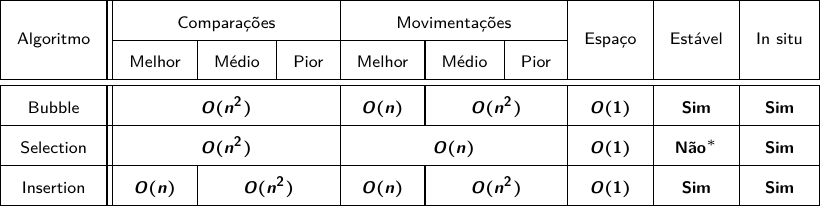
\includegraphics[width=300pt]{imgs/quadro_comparativo.png}
  \label{fig_quadro_comparativo}
\end{figure}
\Tiny{* Existem versões estáveis.}
\end{frame}

%%%%%%%%%%%%%%%%%%%%%%%%%%%%%%%%%%%%%%%%%%%%%%%%%%%%%%%%%%%%%%%%%%%%%%%%%%%%%%%%%%%%%%%%%

\begin{frame}
\frametitle{Conclusão}
\begin{block}{Ordenação}
  \begin{itemize}
   \item A tarefa de ordenação é muito importante, ela é uma necessidade básica para a solução de muitos problemas.
   \item \citeonline{Piva2014} sugere alguns materiais para reforçarem o aprendizagem:
      \begin{itemize}
       \item \href{http://www.inf.ufrgs.br/~bsguedes/simulador/}{Simulador didático de testes de algoritmos de ordenação}
       \item \href{http://www.youtube.com/watch?v=YKlDz1J3TSw}{Vídeo demonstrando os métodos de ordenação}
      \end{itemize}

  \end{itemize}  
\end{block}
\begin{block}{Próxima aula}
  Estudar os algoritmos considerados eficientes.
\end{block}
\end{frame}

%%%%%%%%%%%%%%%%%%%%%%%%%%%%%%%%%%%%%%%%%%%%%%%%%%%%%%%%%%%%%%%%%%%%%%%%%%%%%%%%%%%%%%%%%

\begin{frame}
\Huge{\centerline{Dúvidas}}

\begin{figure}[!h]
  \centering
  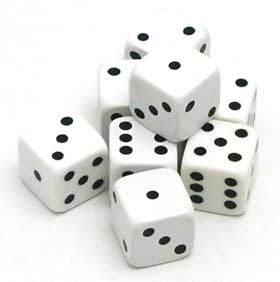
\includegraphics[width=100pt]{imgs/dados.jpg}
  \label{fig_fim}
\end{figure}
\end{frame}
%%%%%%%%%%%%%%%%%%%%%%%%%%%%%%%%%%%%%%%%%%%%%%%%%%%%%%%%%%%%%%%%%%%%%%%%%%%%%%%%%%%%%%%%%
\end{document} 